\let\negmedspace\undefined
\let\negthickspace\undefined
\documentclass[journal]{IEEEtran}
\usepackage[a5paper, margin=10mm, onecolumn]{geometry}
\usepackage{tfrupee} 

\setlength{\headheight}{1cm} 
\setlength{\headsep}{0mm}     

\usepackage{gvv-book}
\usepackage{gvv}
\usepackage{cite}
\usepackage{amsmath,amssymb,amsfonts,amsthm}
\usepackage{algorithmic}
\usepackage{graphicx}
\usepackage{textcomp}
\usepackage{xcolor}
\usepackage{txfonts}
\usepackage{listings}
\usepackage{enumitem}
\usepackage{mathtools}
\usepackage{gensymb}
\usepackage{comment}
\usepackage[breaklinks=true]{hyperref}
\usepackage{tkz-euclide} 
\usepackage{listings}
\def\inputGnumericTable{}                                 
\usepackage[latin1]{inputenc}                                
\usepackage{color}                                            
\usepackage{array}                                            
\usepackage{longtable}                                       
\usepackage{calc}                                             
\usepackage{multirow}                                         
\usepackage{hhline}                                           
\usepackage{ifthen}                                           
\usepackage{lscape}
\usepackage{circuitikz}

\tikzstyle{block} = [rectangle, draw, fill=blue!20, 
    text width=4em, text centered, rounded corners, minimum height=3em]
\tikzstyle{sum} = [draw, fill=blue!10, circle, minimum size=1cm, node distance=1.5cm]
\tikzstyle{input} = [coordinate]
\tikzstyle{output} = [coordinate]

\begin{document}

\bibliographystyle{IEEEtran}
\vspace{3cm}

\title{4.13.18}
\author{EE25BTECH11013 - Bhargav}
\maketitle
{\let\newpage\relax\maketitle}

\renewcommand{\thefigure}{\theenumi}
\renewcommand{\thetable}{\theenumi}
\setlength{\intextsep}{10pt} 

\numberwithin{equation}{enumi}
\numberwithin{figure}{enumi}
\renewcommand{\thetable}{\theenumi}
\textbf{Question}:\\
The line $L$ is given by $\frac{x}{5} + \frac{y}{b} = 1$ passes through the point \brak{13,32}. The line $K$ is parallel to the line $L$ and has the equation $\frac{x}{c} + \frac{y}{3} = 1$. Then the distance between $L$ and $K$ is



\solution \\

The equation of line:
\begin{align}
\vec{n^T}\vec{x} = 1
\end{align}

Line $L$:
\begin{align}
    \myvec{\frac{1}{5} & \frac{1}{b}} \myvec{x \\ y} &= 1
\end{align}

Line $L$ passes through $\myvec{13 \\ 32}$:
\begin{align}
\myvec{\frac{1}{5} & \frac{1}{b}} \myvec{13 \\ 32} &= 1 
\end{align}
\begin{align}
\frac{32}{b} &= 1 - \frac{13}{5}  \implies b=-20
\end{align}



Line $K$:
\begin{align}
    \myvec{\frac{1}{c} & \frac{1}{3}} \myvec{x \\ y} &= 1
\end{align}

Since lines $L$ and $K$ are parallel:
\begin{align}
    \vec{n}_K &= \lambda \vec{n}_L \\
    \myvec{\frac{1}{c} \\ \frac{1}{3}} &= \lambda \myvec{\frac{1}{5} \\ -\frac{1}{20}}
\end{align}

Thus,
\begin{align}
\lambda = -\frac{20}{3} \quad
c = -\frac{3}{4}
\end{align}

\begin{align}
\vec{n} = \myvec{4 \\ -1}
\end{align}
The distance between parallel lines:
\begin{align}
\text{Distance} &= \frac{\abs{c_1 - c_2}}{\norm{\vec{n}}} 
\end{align}

\begin{align}
\text{Distance} &= \frac{\abs{20 - (-3)}}{\sqrt{4^2 + \brak{-1}^2}}
\end{align}

\begin{align}
\therefore \text{Distance} &= \frac{23}{\sqrt{17}}
\end{align}

\begin{figure}[h!]
    \centering
    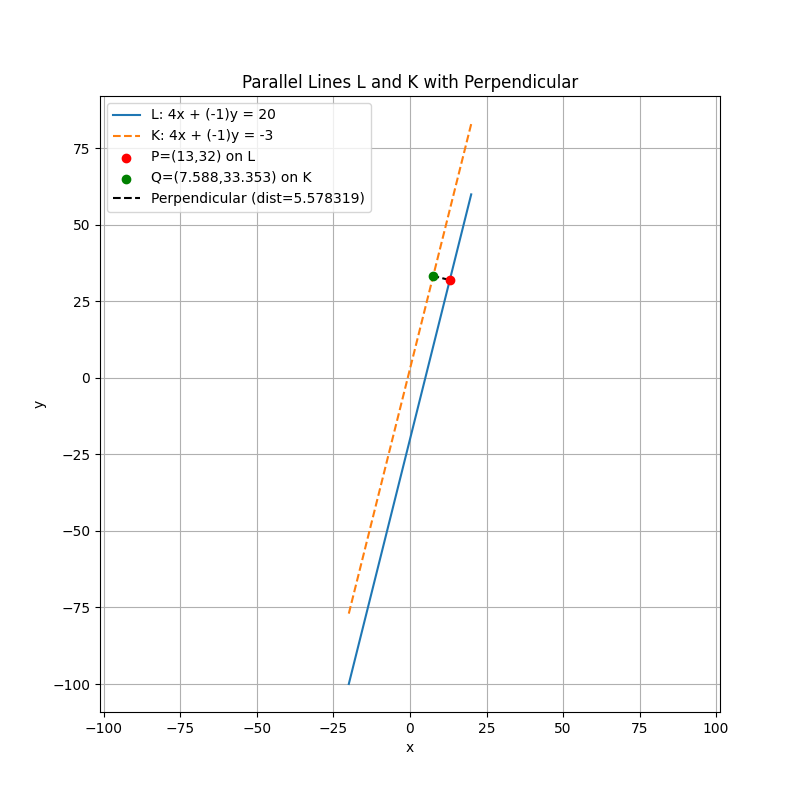
\includegraphics[height=0.5\textheight, keepaspectratio]{figs/Figure_1.png}
    \label{figure_1}
\end{figure}

\end{document}
